\section{Model Following Control}

\subsection{Overview}
%_______________________________________________________________________%
\begin{frame}{Control Loop}
    \begin{figure}[htb]
        \caption{Model Following control block diagram with model control loop process and control loop \cite{Willkomm2023MFC}}
        \label{fig:MFC Control Loop}
        \centering
        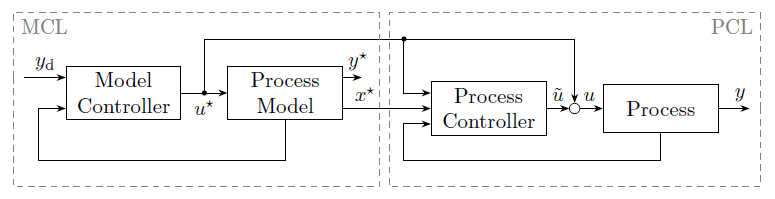
\includegraphics[width=0.8\textwidth]{imgs/MFC/MFC_scheme.PNG}
        \end{figure}
\end{frame}

%_______________________________________________________________________%
\begin{frame}{General Equation}
Consider the flat system : 
\begin{equation}
\label{eq:flat_sys_reduced}
\left\{
\begin{aligned}
  \dot{\xi} &= A\xi + B\big(a(\xi) + b(\xi)u + \Delta(\xi, t) \big) \\
  y &= C\xi
\end{aligned}
\right.
\end{equation}



where  and \( \xi(t) \in \mathbb{D}_\xi \subseteq \mathbb{R}^n \) denote the states. 
\(\Delta: \mathbb{D}_{\xi} \times \mathbb{R}^+ \rightarrow \mathbb{R}\) are the perturbations. \\
The output is \( y(t) \in \mathbb{R} \) and \( u(t) \in \mathbb{R} \) denotes the input. The relative degree is \( n \ge 1 \). 

 \begin{block}{Remark}
    Here we consider a SISO system. That doesn't matter as the crane's 3 outputs are decoupled. The control loop can be separated into 3 distinct SISO control loops of dimension 4.
    \end{block}

\end{frame}

\begin{frame}{General Equation}
The matrices \( A \), \( B \), and \( C \) are given by:

\begin{align*}
A &=
\begin{bmatrix}
0 & 1 & 0 & \cdots & 0 \\
0 & 0 & 1 & \cdots & 0 \\
\vdots & \vdots & \ddots & \ddots & \vdots \\
0 & 0 & \cdots & 0 & 1 \\
0 & 0 & \cdots & 0 & 0
\end{bmatrix}
\in \mathbb{R}^{n \times n}, \quad
B =
\begin{bmatrix}
0 \\
0 \\
\vdots \\
0 \\
1
\end{bmatrix}
\in \mathbb{R}^n, \\
C &=
\begin{bmatrix}
1 & 0 & \cdots & 0
\end{bmatrix}
\in \mathbb{R}^{1 \times n}
\end{align*}
\end{frame}


%_______________________________________________________________________%
\subsection{Model Control Loop (MCL)}
\begin{frame}{MCL Dynamics}
    An analysis of the control loop dynamics can be carried out in two stages. First, we consider the Model Control Loop (MCL), which is a replica of system \ref{eq:flat_sys_reduced}, excluding the perturbations \(\Delta\), and is described by:

\begin{equation}
\label{eq:MCL_open_loop}
  \dot{\xi^*} = A\xi^* + B\big(a(\xi^*) + b(\xi^*)u^* \big)
\end{equation}

\end{frame}

\begin{frame}{Open Loop dynamics}
    We write :  \(u = \tilde{u} + u^*\), where \(u^*\) : the output of the MCL and \(\tilde{u}\) : the output of the process control loop \\
    The error states are defined as \(\tilde{\xi} = \xi - \xi^*\), and the open-loop dynamics of the MFC are given by:

\begin{align}
\dot{\xi}^* &= A\xi^* + B \left( a(\xi^*) + b(\xi^*) u^* \right) \\
\dot{\tilde{\xi}} &= A\tilde{\xi} + B \left( \tilde{a}(\xi^*, \tilde{\xi}, u^*) + b(\xi^* + \tilde{\xi}) \tilde{u} + \Delta(\xi^* + \tilde{\xi}, t)  \right)
\end{align}

where

\begin{align}
\tilde{a}(\xi^*, \tilde{\xi}, u^*) &= a(\xi^* + \tilde{\xi}) - a(\xi^*) + \left( b(\xi^* + \tilde{\xi}) - b(\xi^*) \right) u^*
\end{align}


\end{frame}


\begin{frame}{Feedback Linearization}
    
Ensure closed-loop stability : a feedback linearization law is applied to the MCL  defined by:

\begin{equation}
\label{eq:MCL_control_law}
u^* = -\frac{a(\xi^*) + v^*}{b(\xi^*)}
\end{equation}

The design of \(v^*\) is based on the error dynamics within the MCL : \(\tilde{\xi}^* = \xi^* - \xi_d\) representing the deviation between the model and desired states. The associated error dynamics are given by:

\begin{align}
\dot{\tilde{\xi}}^* &= A\tilde{\xi}^* + B(v^* - y_d^{(r)})
\end{align}

\end{frame}



\begin{frame}{Closed Loop Dynamics}
The new input \(v^*\) is chosen as:

\begin{equation}
v^* = y_d^{(r)} + K\tilde{\xi}^*
\end{equation}

where \(K = [-\alpha_0, -\alpha_1, \ldots, -\alpha_{r-1}] \in \mathbb{R}^{1 \times r}\) is selected such that the matrix \(A + BK\) is Hurwitz. The closed-loop dynamics of the MCL become:

\begin{align}
\dot{\tilde{\xi}}^* &= (A + BK)\tilde{\xi}^*
\end{align}
\end{frame}


%_______________________________________________________________________%

\subsection{Process Control Loop (PCL)}
\begin{frame}{Introduction}
    The process control loop is design to counter the perturbations and model uncertainties. The design method to assure robustness is the high-control gain approach. The desired output trajectory \(y_d(t) \in \mathbb{R}\) is assumed to be at least n-times continuously differentiable. The desired external states \(\xi_d(t) \in \mathbb{D}_{\xi_d}  \subseteq \mathbb{R}^n\) are generated by 

\begin{equation}
    \dot{\xi_d} = A\xi_d + By_d^{(n)}
\end{equation}

\end{frame}

\begin{frame}{Open Loop Dynamics}
    The open-loop error dynamics :

\begin{align}
\dot{\tilde{\xi}} &= A\tilde{\xi} + B\left(\tilde{a}(\xi^*, \tilde{\xi}, u^*) + b(\tilde{\xi}^* + \tilde{\xi}) \tilde{u} + \Delta(\tilde{\xi}^* + \tilde{\xi}, t) \right)
\end{align}

The design of the process controller will also be a feedback linearizing control law :

\begin{equation}
\tilde{u} = \frac{-\tilde{a}(\xi^*, \tilde{\xi}, u^*) + \tilde{K}\tilde{\xi}}{b(\xi^* + \xi)}
\end{equation}

where : \(\tilde{K} = KD^{-1}\varepsilon^{-1}\) with \(D = \text{diag}(\varepsilon^{n}, \varepsilon^{n-1}, \ldots, 1)\) and \(0 < \varepsilon < 1\) is a time scaling parameter.

\end{frame}

\begin{frame}{Overall Dynamics}
    
We proceed the time scaling change of variable : 

\begin{equation}
    \zeta = D^{-1}\tilde{\xi}
\end{equation}

The closed-loop overall dynamics of the MFC scheme for set-point and trajectory tracking are given by

\begin{align}
\label{eq:The closed-loop overall dynamics of the MFC}
\dot{\tilde{\xi}}^* &= (A + BK)\tilde{\xi}^* \\
\varepsilon\dot{\zeta} &= (A + BK)\zeta + \varepsilon B \left(\Delta(\xi_d + \tilde{\xi}^* + D\zeta, t) \right).
\end{align}

\end{frame}

\begin{frame}{Process Control Loop}
    \begin{itemize}
    \item If \( A + BK \) is Hurwitz, the eigenvalues of the error dynamics (without time-scaling) can be shifted arbitrarily far to the left of the imaginary axis as \( \epsilon \rightarrow 0 \).
    \item Theoretically, the error dynamics can be made to converge arbitrarily quickly.
    \item Achieving this may necessitate a significantly large control effort.
    \item A small \( \epsilon \) enhances robustness against perturbations \( \Delta(\xi, t) \). One can with this assumption : 
    \[
    |\Delta(\xi, t)| \leq \delta + L_\Delta \lVert \xi \rVert_2
    \]
    Find a condition on \(\epsilon\) to encounter the perturbations.
    \item Additionally, a small \( \epsilon \) accelerates the error dynamics of the PCL.
\end{itemize}
\end{frame}



%_______________________________________________________________________%
\begin{frame}{A Simpler Design}
\cite{Tietze2023CruiseControl} showed a simpler architecture of the MFC, which includes the following key points:

\begin{itemize}
    \item The feedback linearization control law is given by:
    \(
    u = \frac{-a(\xi) + y_d^{(n)} + v}{b(\xi)}
    \)
    where \( v = v^* + \tilde{v} \).

    \item The dynamics of the open loop are described by:
    \[
    \dot{\xi} = A\xi + B(y_d^{(n)} + v) + \Delta(\xi, t)
    \]

    \item The nominal model of the external dynamics is given by the integrator chain:
    \[
    \dot{\xi}^* = A\xi^* + B(y_d^{(n_\xi)} + v^*)
    \]
    with the initial state \(\xi^*(0) = \xi_0^*\), and the error dynamics:
    \[
    \dot{\tilde{\xi}} = A\tilde{\xi} + B(\tilde{v} + \Delta(\xi, \eta, t))
    \]
\end{itemize}
\end{frame}

\begin{frame}{A Simpler Design}
\cite{Tietze2023CruiseControl} continued:

\begin{itemize}
    \item The dynamics of the open-loop MFC system include:
 \begin{align}
    \dot{\tilde{\xi}}^* &= A\tilde{\xi}^* + Bv^* \\
    \dot{\tilde{\xi}} &= A\tilde{\xi} + B(\tilde{v} + \Delta(\xi, t))
 \end{align}
    
    \item One can rewrite the control loop as follows : 

    \begin{figure}
        \centering
        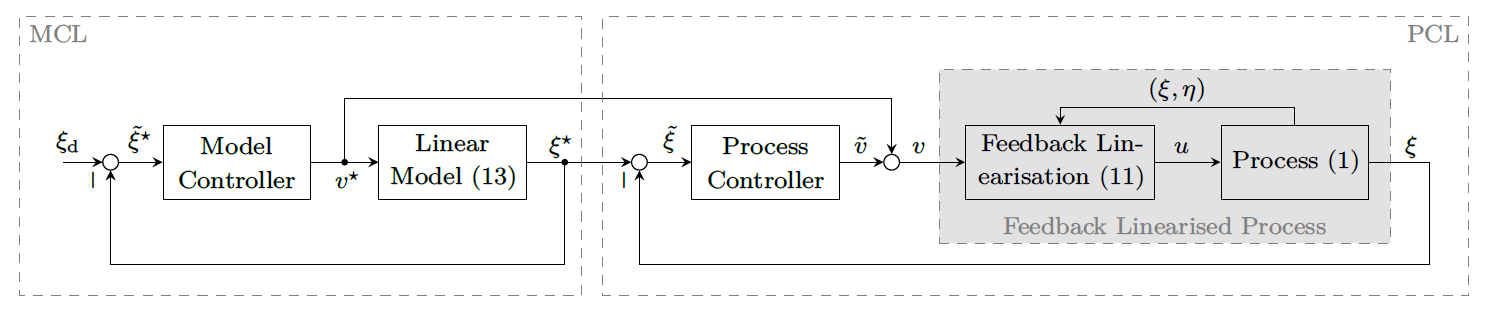
\includegraphics[width=0.9\linewidth]{imgs/MFC/MFCEfficient.PNG}
        \caption{Block-diagram of the MFC architecture with linear model of the feedback linearized process \cite{Tietze2023CruiseControl}}
        \label{fig:Blockdiagram of the MFC architecture with linear model of the feedback linearised process}
    \end{figure}

\end{itemize}
\end{frame}

\begin{frame}{Control Loops Comparison}
    \begin{figure}
        \centering
        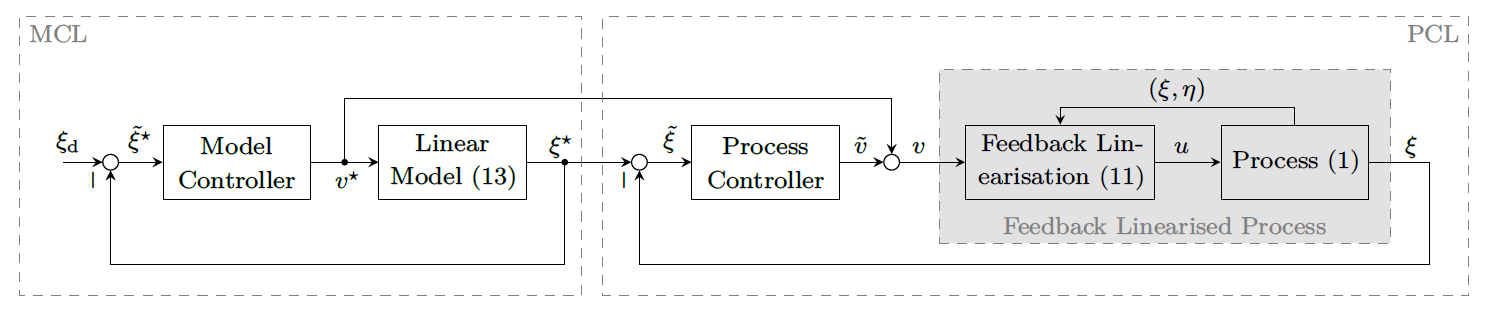
\includegraphics[width=0.9\linewidth]{imgs/MFC/MFCEfficient.PNG}
        
        \label{fig:Blockdiagram of the MFC architecture with linear model of the feedback linearised process}
    \end{figure}

     \begin{figure}
       
        \label{fig:MFC Control Loop}
        \centering
        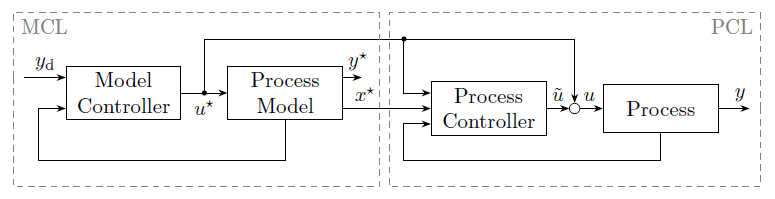
\includegraphics[width=0.9\textwidth]{imgs/MFC/MFC_scheme.PNG}
     \end{figure}

    
\end{frame}


%_______________________________________________________________________%

\subsection{High Gain Control Comparison}
\begin{frame}{High Gain Control}

The High Gain Control law is formulated as:

\begin{equation}
u = \frac{-a(\xi) + K_\epsilon \xi }{b(\xi)}
\end{equation}

\begin{itemize}
    \item With only one loop in the control. The slower motion of the MCL are not present and the PCL alone try to stabilize the dynamics.

    \item This control law is designed to aggressively reduce the error, leading to rapid convergence to the desired state.
\end{itemize}

\end{frame}


\begin{frame}{Peaking Phenomenon}
    
However, it is clear that we have peaking with this method, which is characterized by:

\begin{block}{Peaking Phenomenon}
Peaking refers to large transient peaks in control signals or state variables, caused by high gain amplifying initial errors or disturbances. This can lead to:
\begin{itemize}
    \item Large temporary deviations in system response.
    \item Potential saturation of actuators, resulting in performance degradation or instability.
    \item Challenges in systems with fast dynamics or constrained states.
\end{itemize}
\end{block}

\end{frame}


